\documentclass[../main.tex]{subfiles}

\graphicspath{ {images/}{../images/} }

\begin{document}
    W badaniu porównane zostaną wyniki procesu wykrywania podobieństwa obrazów z uwzględnieniem wniosków cząstkowych uzyskanych w poprzednich etapach. Otrzymane rezultaty zostaną porównane z uruchomieniem metody bez uwzględniania wniosków cząstkowych. W przypadku obu uruchomień wykorzystana zostanie metoda estymacji liczby wymaganych iteracji, w celu przyśpieszenia obliczeń, oraz transformata perspektywiczna. 
    \begin{figure}[H]
     \begin{center}
     \caption{Tabela z parametrami uruchomieniowymi}
      \begin{tabular}{|c|c|c|c|c|c|}
      \hline
      \thead{Instancja} & \thead{Liczność sąsiedztwa} & \thead{Próg spójności} & \thead{Heurystyka} & \thead{Maksymalny \\ błąd modelu} \\
      \hline
      
      {Z uwzględnieniem wniosków} & \makecell{}{50} & \makecell{}{0.5} & {Odległość punktów} & \makecell{}{20} \\
      \hline
      {Bez  uwzględniania} & \makecell{}{10} & \makecell{}{0.7} & {Losowanie} & \makecell{}{40} \\
      \hline

      \end{tabular}
     \end{center}
    \end{figure}
    
    \begin{figure}[H]
        \centering
        \begin{minipage}{.5\textwidth}
            \caption{Wynik z dobrymi paramterami}
            \centering
            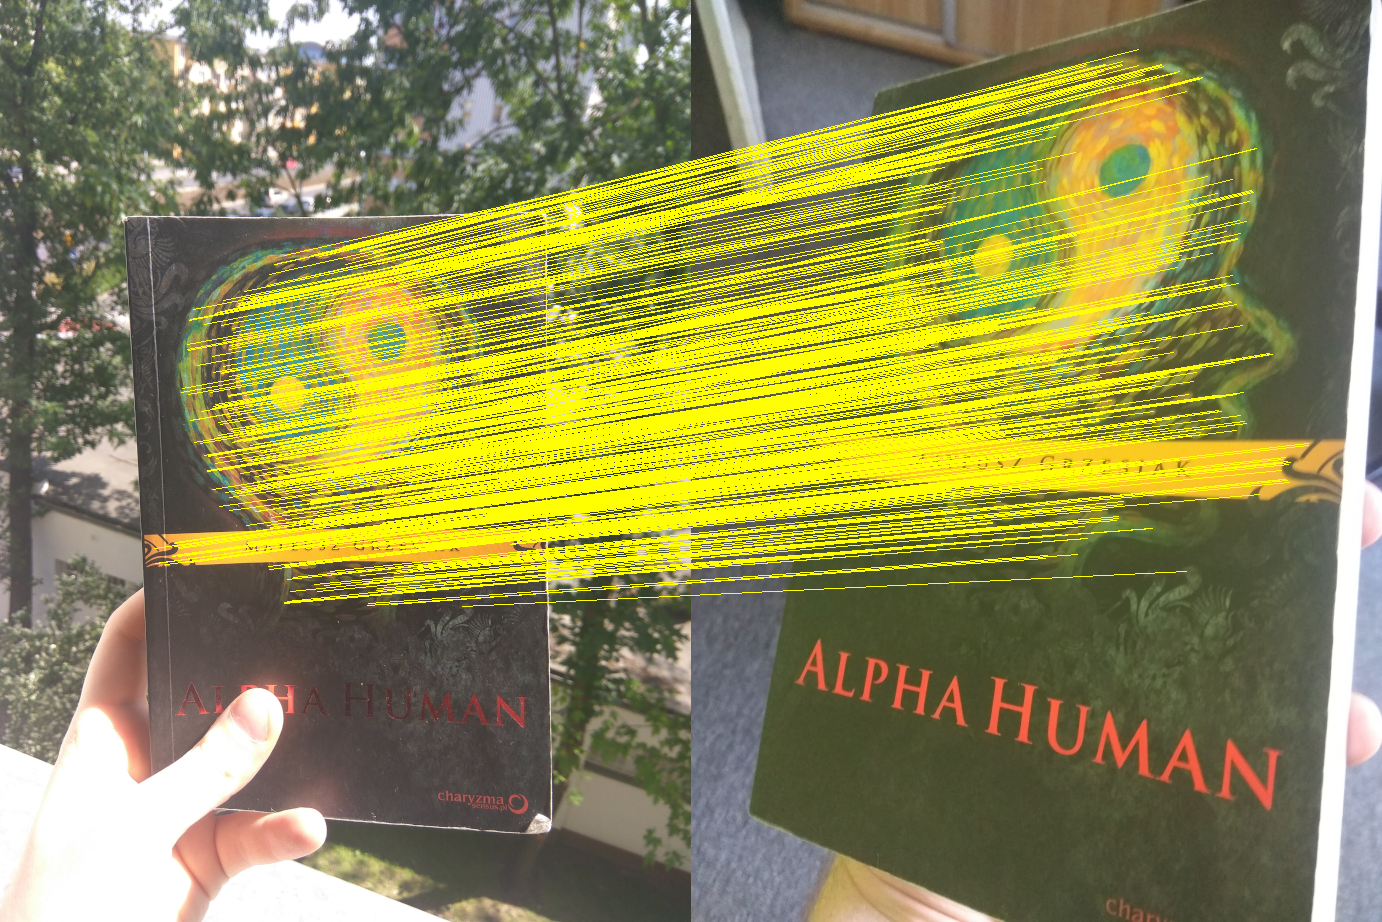
\includegraphics[width=7cm]{final_test_good}
        \end{minipage}%
        \begin{minipage}{.5\textwidth}
            \caption{Wynik ze złymi parametrami}
            \centering
            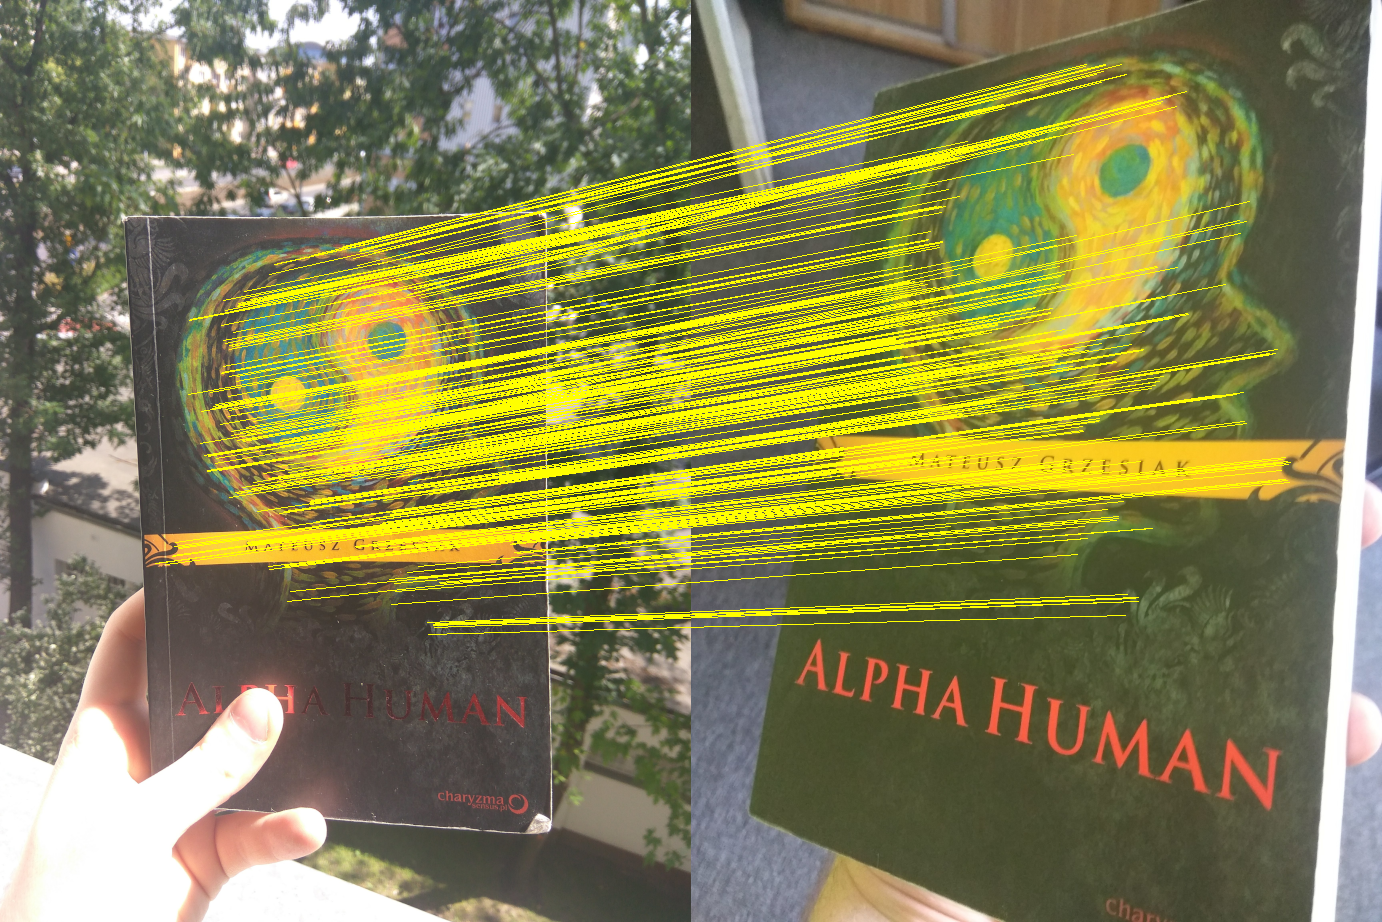
\includegraphics[width=7cm]{final_test_bad}
        \end{minipage}%
    \end{figure}

        \begin{figure}[H]
     \begin{center}
     \caption{Tabela wynikowa}
      \begin{tabular}{|c|c|c|c|c|c|}
      \hline
      \thead{Instancja} & \thead{Liczba \\ par \\ spójnych} & \thead{Najlepszy \\ wynik} & \thead{Znaleziony \\w iteracji nr} & \thead{Całkowita \\ liczba \\ iteracji} & \thead{Czas \\ przetwarzania [s]} \\
      \hline
      
      {Z uwzględnieniem wniosków} & \makecell{}{650} 
      & \makecell{}{636} & \makecell{}{38} 
      & \makecell{}{38} & \makecell{}{0,85} \\
      \hline
      {Bez  uwzględniania} & \makecell{}{353} 
      & \makecell{}{353} & \makecell{}{11} 
      & \makecell{}{445} & \makecell{}{7,29} \\
      \hline

      \end{tabular}
     \end{center}
    \end{figure}

    \paragraph{}
    Jak można zauważyć uruchomienie algorytmu po uwzględnieniu wniosków cząstkowych z poprzednich etapów pozwoliło na osiągnięcie prawie dwukrotnie lepszego rezultatu pod względem liczby par punktów kluczowych. Różnica czasowa także jest znaczna, wystrojony algorytm dokonał swoich obliczeń ponad osiem razy szybciej. Na czas działania napewno miała wpływ liczba par spójnych, która jest wykorzystywana w metodzie estymacji iteracji wymaganych do znalezienia odpowiedniego modelu.
    
    \paragraph{}
    Na zdjęciach widać, że choć uruchomienie algorytmu z niezbyt dobrymi algorytmami wypada gorzej od uwzględnienia wniosków cząstkowych, to nadal wynik jest dobry. Gorszy wynik wynika głównie z faktu, że w trakcie badania spójności par punktów, usuniętych zostało dużo par poprawnych. Można także zauważyć, że w obu przypadkach algorytm skupił się na tylko i wyłącznie na logo książki, wynika to zapewne z faktu, że reszta okładki jest dosyć ciemna, więc skrypt do wyznaczanie punktów spójnych te regiony poprostu pominął.
    
\end{document}
